\documentclass[11pt,a4paper]{report}
\usepackage[textwidth=37em,vmargin=30mm]{geometry}
\usepackage{calc,xunicode,amsmath,amssymb,paralist,enumitem,tabu,booktabs,datetime2,xeCJK,xeCJKfntef,listings}
\usepackage{tocloft,fancyhdr,tcolorbox,xcolor,graphicx,eso-pic,xltxtra,xelatexemoji}

\newcommand{\envyear}[0]{2025}
\newcommand{\envdatestr}[0]{2025-10-23}
\newcommand{\envfinaldir}[0]{webdb/2025/20251023/final}

\usepackage[hidelinks]{hyperref}
\hypersetup{
    colorlinks=false,
    pdfpagemode=FullScreen,
    pdftitle={Web Digest - \envdatestr}
}

\setlength{\cftbeforechapskip}{10pt}
\renewcommand{\cftchapfont}{\rmfamily\bfseries\large\raggedright}
\setlength{\cftbeforesecskip}{2pt}
\renewcommand{\cftsecfont}{\sffamily\small\raggedright}

\setdefaultleftmargin{2em}{2em}{1em}{1em}{1em}{1em}

\usepackage{xeCJK,xeCJKfntef}
\xeCJKsetup{PunctStyle=plain,RubberPunctSkip=false,CJKglue=\strut\hskip 0pt plus 0.1em minus 0.05em,CJKecglue=\strut\hskip 0.22em plus 0.2em}
\XeTeXlinebreaklocale "zh"
\XeTeXlinebreakskip = 0pt


\setmainfont{Brygada 1918}
\setromanfont{Brygada 1918}
\setsansfont{IBM Plex Sans}
\setmonofont{JetBrains Mono NL}
\setCJKmainfont{Noto Serif CJK SC}
\setCJKromanfont{Noto Serif CJK SC}
\setCJKsansfont{Noto Sans CJK SC}
\setCJKmonofont{Noto Sans CJK SC}

\setlength{\parindent}{0pt}
\setlength{\parskip}{8pt}
\linespread{1.15}

\lstset{
	basicstyle=\ttfamily\footnotesize,
	numbersep=5pt,
	backgroundcolor=\color{black!5},
	showspaces=false,
	showstringspaces=false,
	showtabs=false,
	tabsize=2,
	captionpos=b,
	breaklines=true,
	breakatwhitespace=true,
	breakautoindent=true,
	linewidth=\textwidth
}






\newcommand{\coverpic}[2]{
    % argv: itemurl, authorname
    Cover photo by #2~~(\href{#1}{#1})
}
\newcommand{\makeheader}[0]{
    \begin{titlepage}
        % \newgeometry{hmargin=15mm,tmargin=21mm,bmargin=12mm}
        \begin{center}
            
            \rmfamily\scshape
            \fontspec{BaskervilleF}
            \fontspec{Old Standard}
            \fontsize{59pt}{70pt}\selectfont
            WEB\hfill DIGEST
            
            \vfill
            % \vskip 30pt
            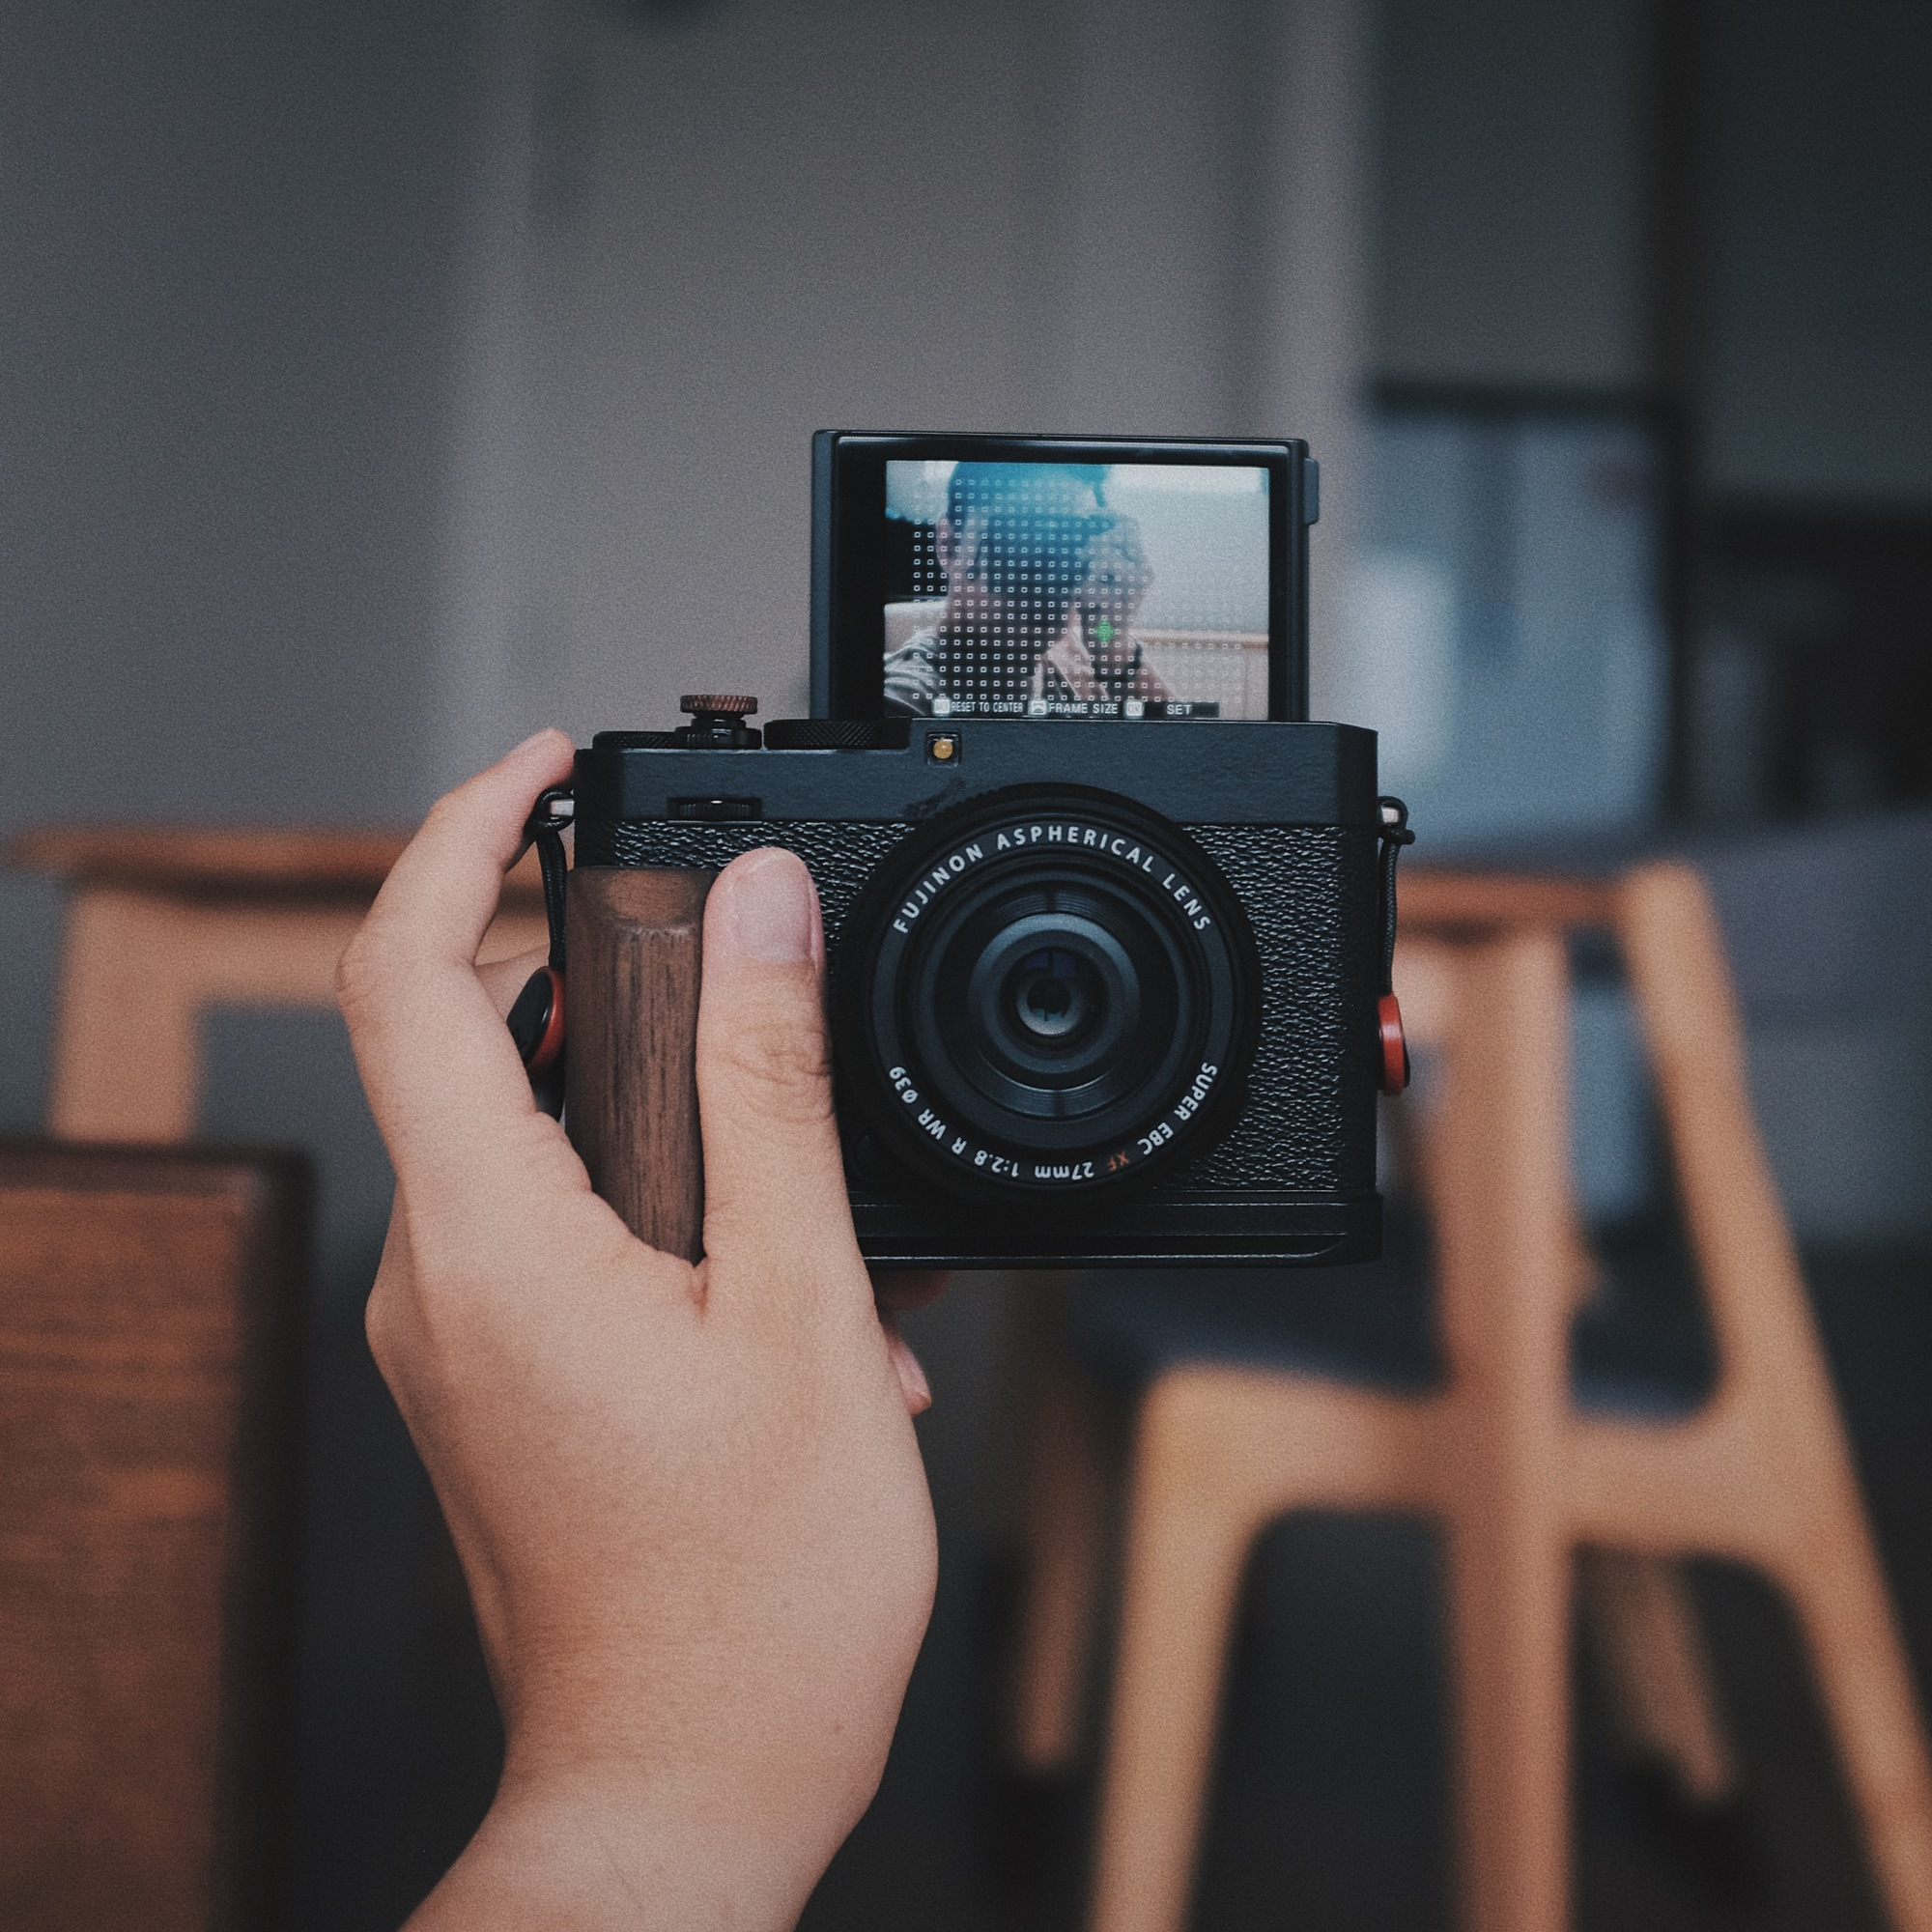
\includegraphics[width=\linewidth]{\envfinaldir/coverpic-prod.jpg}\par
            % \vskip 30pt
            \vfill

            \normalsize\rmfamily\scshape
            \copyright{} The Web Digest Project \hfill\large \envdatestr
        \end{center}
    \end{titlepage}
    % \restoregeometry
}
\newcommand{\simplehref}[1]{%
    \textcolor{blue!80!green}{\href{#1}{#1}}%
}
\renewcommand{\contentsname}{\center\Huge\sffamily\bfseries Contents\par\vskip 20pt}
\newcounter{ipartcounter}
\setcounter{ipartcounter}{0}
\newcommand{\ipart}[1]{
    % \vskip 20pt
    \clearpage
    \stepcounter{ipartcounter}
    \phantomsection
    \addcontentsline{toc}{chapter}{#1}
    % \begin{center}
    %     \Huge
    %     \sffamily\bfseries
    %     #1
    % \end{center}
    % \vskip 20pt plus 7pt
}
\newcounter{ichaptercounter}
\setcounter{ichaptercounter}{0}
\newcommand{\ichapter}[1]{
    % \vskip 20pt
    \clearpage
    \stepcounter{ichaptercounter}
    \phantomsection
    \addcontentsline{toc}{section}{\numberline{\arabic{ichaptercounter}}#1}
    \begin{center}
        \Huge
        \sffamily\bfseries
        #1
    \end{center}
    \vskip 20pt plus 7pt
}
\newcommand{\entrytitlefont}[1]{\subsection*{\raggedright\Large\sffamily\bfseries#1}}
\newcommand{\entryitemGeneric}[2]{
    % argv: title, url
    \parbox{\linewidth}{
        \entrytitlefont{#1}\par\vskip 5pt
        \footnotesize\ttfamily\mdseries
        \simplehref{#2}
    }\vskip 11pt plus 11pt minus 1pt
}
\newcommand{\entryitemGithub}[3]{
    % argv: title, url, desc
    \parbox{\linewidth}{
        \entrytitlefont{#1}\par\vskip 5pt
        \footnotesize\ttfamily\mdseries
        \simplehref{#2}\par\vskip 5pt
        \small\rmfamily\mdseries#3
    }\vskip 11pt plus 11pt minus 1pt
}
\newcommand{\entryitemAp}[3]{
    % argv: title, url, desc
    \parbox{\linewidth}{
        \entrytitlefont{#1}\par\vskip 5pt
        \footnotesize\ttfamily\mdseries
        \simplehref{#2}\par\vskip 5pt
        \small\rmfamily\mdseries#3
    }\vskip 11pt plus 11pt minus 1pt
}
\newcommand{\entryitemHackernews}[3]{
    % argv: title, hnurl, rawurl
    % \parbox{\linewidth}{
    %     \entrytitlefont{#1}\par\vskip 5pt
    %     \footnotesize\ttfamily\mdseries
    %     \simplehref{#3}\par
    %     \textcolor{black!50}{\href{#2}{#2}}
    % }\vskip 11pt plus 11pt minus 1pt
    \begin{minipage}{\linewidth}
            \entrytitlefont{#1}\par\vskip 5pt
            \footnotesize\ttfamily\mdseries
            \simplehref{#3}\par
            \textcolor{black!50}{\href{#2}{#2}}
    \end{minipage}\par\vskip 11pt plus 11pt minus 1pt
}







\begin{document}

\makeheader

\tableofcontents\clearpage




\ipart{Developers}
\ichapter{Hacker News}
\entryitemTwoLinks{Ovi: Twin backbone cross-modal fusion for audio-video generation}{https://news.ycombinator.com/item?id=45674166}{https://github.com/character-ai/Ovi}

\entryitemTwoLinks{ROG Xbox Ally runs better on Linux than Windows it ships with}{https://news.ycombinator.com/item?id=45673542}{https://www.tomshardware.com/video-games/handheld-gaming/rog-xbox-ally-runs-better-on-linux-than-the-windows-it-ships-with-new-test-shows-up-to-32-percent-higher-fps-with-more-stable-framerates-and-quicker-sleep-resume-times}

\entryitemTwoLinks{Criticisms of ``The Body Keeps the Score''}{https://news.ycombinator.com/item?id=45673479}{https://josepheverettwil.substack.com/p/the-body-keeps-the-score-is-bullshit}

\entryitemTwoLinks{Mass Assignment Vulnerability Exposes Max Verstappen Passport and F1 Drivers PII}{https://news.ycombinator.com/item?id=45673130}{https://ian.sh/fia}

\entryitemTwoLinks{Rivian's TM-B electric bike}{https://news.ycombinator.com/item?id=45672844}{https://www.theverge.com/news/804157/rivian-tm-b-electric-bike-price-specs-helmet-quad}

\entryitemTwoLinks{JMAP for Calendars, Contacts and Files Now in Stalwart}{https://news.ycombinator.com/item?id=45672336}{https://stalw.art/blog/jmap-collaboration/}

\entryitemTwoLinks{I see a future in jj}{https://news.ycombinator.com/item?id=45672280}{https://steveklabnik.com/writing/i-see-a-future-in-jj/}

\entryitemTwoLinks{HP SitePrint}{https://news.ycombinator.com/item?id=45672235}{https://www.hp.com/us-en/printers/site-print/layout-robot.html}

\entryitemTwoLinks{Look, Another AI Browser}{https://news.ycombinator.com/item?id=45672199}{https://manuelmoreale.com/thoughts/look-another-ai-browser}

\entryitemTwoLinks{Galaxy XR: The first Android XR headset}{https://news.ycombinator.com/item?id=45671871}{https://blog.google/products/android/samsung-galaxy-xr/}

\entryitemTwoLinks{Meta is axing 600 roles across its AI division}{https://news.ycombinator.com/item?id=45671778}{https://www.theverge.com/news/804253/meta-ai-research-layoffs-fair-superintelligence}

\entryitemTwoLinks{Willow quantum chip demonstrates verifiable quantum advantage on hardware}{https://news.ycombinator.com/item?id=45670443}{https://blog.google/technology/research/quantum-echoes-willow-verifiable-quantum-advantage/}

\entryitemTwoLinks{Scripts I wrote that I use all the time}{https://news.ycombinator.com/item?id=45670052}{https://evanhahn.com/scripts-i-wrote-that-i-use-all-the-time/}

\entryitemTwoLinks{Cryptographic Issues in Cloudflare's Circl FourQ Implementation (CVE-2025-8556)}{https://news.ycombinator.com/item?id=45669593}{https://www.botanica.software/blog/cryptographic-issues-in-cloudflares-circl-fourq-implementation}

\entryitemTwoLinks{Linux Capabilities Revisited}{https://news.ycombinator.com/item?id=45669142}{https://dfir.ch/posts/linux\_capabilities/}

\entryitemTwoLinks{AI assistants misrepresent news content 45\% of the time}{https://news.ycombinator.com/item?id=45668990}{https://www.bbc.co.uk/mediacentre/2025/new-ebu-research-ai-assistants-news-content}

\entryitemTwoLinks{Democracy and the open internet die in daylight}{https://news.ycombinator.com/item?id=45668453}{https://heatherburns.tech/2025/10/22/democracy-and-the-open-internet-die-in-daylight/}

\entryitemTwoLinks{The Dragon Hatchling: The missing link between the transformer and brain models}{https://news.ycombinator.com/item?id=45668408}{https://arxiv.org/abs/2509.26507}

\entryitemTwoLinks{The security paradox of local LLMs}{https://news.ycombinator.com/item?id=45668264}{https://quesma.com/blog/local-llms-security-paradox/}

\entryitemTwoLinks{SourceFS: A 2h+ Android build becomes a 15m task with a virtual filesystem}{https://news.ycombinator.com/item?id=45668160}{https://www.source.dev/journal/sourcefs}\ichapter{Phoronix}
\entryitemGeneric{\hskip 0pt{}Google Develops Code Prefetch Insertion Optimizer For Faster Intel GNR \& AMD Turin Performance}{https://www.phoronix.com/news/Propeller-Prefetch-Insertion}

\entryitemGeneric{\hskip 0pt{}Linux 6.19 To Support The XP-PEN Artist 24 Pro Drawing Tablet}{https://www.phoronix.com/news/Linux-6.19-XP-PEN-Artist-24-Pro}

\entryitemGeneric{\hskip 0pt{}Fedora Will Allow AI-Assisted Contributions With Proper Disclosure \& Transparency}{https://www.phoronix.com/news/Fedora-Allows-AI-Contributions}

\entryitemGeneric{\hskip 0pt{}Ray AI Engine Pulled Into The PyTorch Foundation For Unified Open AI Compute Stack}{https://www.phoronix.com/news/PyTorch-Ray-AI-Compute-Engine}

\entryitemGeneric{\hskip 0pt{}Linux 6.18 Hardened Against Specially-Crafted EROFS Images Leading To System Crashes}{https://www.phoronix.com/news/Linux-6.18-EROFS-Hardening}

\entryitemGeneric{\hskip 0pt{}Sovereign Tech Agency Making 2026 Investments In systemd, PHP, Servo \& More}{https://www.phoronix.com/news/STF-2026-systemd-PHP}

\entryitemGeneric{\hskip 0pt{}LLVM Lands Some Long Overdue Tuning Optimizations For AMD Zen 4}{https://www.phoronix.com/news/LLVM-Overdue-Znver4-Tuning}

\entryitemGeneric{\hskip 0pt{}Linux 6.18 Adding AWCC Profile Support For The Dell G15 5530}{https://www.phoronix.com/news/Dell-G15-5530-AWCC-Linux-6.18}

\entryitemGeneric{\hskip 0pt{}Intel Xe3P\_LPD Display Support For Linux Being Built Out Ahead Of Nova Lake}{https://www.phoronix.com/news/Intel-Xe3P-LPD-Display-Linux}


\ipart{Developers~~~~(zh-Hans)}
\ichapter{Solidot}
\entryitemGeneric{\hskip 0pt{}马斯克对 NASA 代理局长宣战}{https://www.solidot.org/story?sid=82608}

\entryitemGeneric{\hskip 0pt{}Valkey 9.0.0 释出}{https://www.solidot.org/story?sid=82607}

\entryitemGeneric{\hskip 0pt{}外国黑客利用 SharePoint 漏洞入侵美国核武器工厂}{https://www.solidot.org/story?sid=82606}

\entryitemGeneric{\hskip 0pt{}OpenAI 发布 AI 浏览器 ChatGPT Atlas}{https://www.solidot.org/story?sid=82605}

\entryitemGeneric{\hskip 0pt{}美国缩小 10 万美元 H-1B 签证费适用范围}{https://www.solidot.org/story?sid=82604}

\entryitemGeneric{\hskip 0pt{}PRIMA 芯片助黄斑变性失明患者恢复视力}{https://www.solidot.org/story?sid=82603}

\entryitemGeneric{\hskip 0pt{}TikTok 修改政策不再提前通知用户政府索要其数据}{https://www.solidot.org/story?sid=82602}

\entryitemGeneric{\hskip 0pt{}盖亚望远镜发现银河系的巨浪}{https://www.solidot.org/story?sid=82601}

\entryitemGeneric{\hskip 0pt{}SpaceX 进度滞后 NASA 可能选择其它公司开发月球着陆器}{https://www.solidot.org/story?sid=82600}

\entryitemGeneric{\hskip 0pt{}美国客机疑与气象气球发生碰撞}{https://www.solidot.org/story?sid=82599}

\entryitemGeneric{\hskip 0pt{}KDE Plasma 6.5 释出}{https://www.solidot.org/story?sid=82598}

\entryitemGeneric{\hskip 0pt{}中国东南沿海同时遭遇海平面加速上升和地面下沉}{https://www.solidot.org/story?sid=82597}

\entryitemGeneric{\hskip 0pt{}被切断大脑区域的脑电图与深度睡眠脑电图相似}{https://www.solidot.org/story?sid=82596}

\entryitemGeneric{\hskip 0pt{}SpaceX 发射了第 1 万颗 Starlink 卫星}{https://www.solidot.org/story?sid=82595}

\entryitemGeneric{\hskip 0pt{}Steam 平台一款游戏的愿望单数字越高是否销量越多?}{https://www.solidot.org/story?sid=82594}

\entryitemGeneric{\hskip 0pt{}零工正在训练会取代他们的技术}{https://www.solidot.org/story?sid=82593}

\entryitemGeneric{\hskip 0pt{}冰岛发现野外蚊子}{https://www.solidot.org/story?sid=82592}

\entryitemGeneric{\hskip 0pt{}FSF 呼吁 Windows 10 用户切换到 GNU/Linux}{https://www.solidot.org/story?sid=82591}

\entryitemGeneric{\hskip 0pt{}韦伯望远镜发现的小红点是什么?}{https://www.solidot.org/story?sid=82590}

\entryitemGeneric{\hskip 0pt{}Servo v0.0.1 释出}{https://www.solidot.org/story?sid=82589}\ichapter{V2EX}
\entryitemGeneric{\hskip 0pt{}[Windows] 最近 windows11 会在早晨自动切换为深色?并且无法改为浅色?}{https://www.v2ex.com/t/1167726}

\entryitemGeneric{\hskip 0pt{}[分享发现] 好看的 IPv6 网络连接检测工具}{https://www.v2ex.com/t/1167725}

\entryitemGeneric{\hskip 0pt{}[分享发现] 有些人完全把本站当成了提现工具}{https://www.v2ex.com/t/1167724}

\entryitemGeneric{\hskip 0pt{}[分享创造] 为了吃饭,来这里拉点人气}{https://www.v2ex.com/t/1167723}

\entryitemGeneric{\hskip 0pt{}[Apple] 果不其然, iPhone Air 扑街了}{https://www.v2ex.com/t/1167722}

\entryitemGeneric{\hskip 0pt{}[iPad] 有没有 mini7 的用户升级了 26 之后速度如何?}{https://www.v2ex.com/t/1167720}

\entryitemGeneric{\hskip 0pt{}[问与答] 求助,我妈上班路上崴脚了,骨折了。}{https://www.v2ex.com/t/1167719}

\entryitemGeneric{\hskip 0pt{}[分享发现] v 友们来大胆猜测这次内存价格会到多少?}{https://www.v2ex.com/t/1167718}

\entryitemGeneric{\hskip 0pt{}[酷工作] 一个奇葩的想法,请教一下各位大佬是否行得通}{https://www.v2ex.com/t/1167716}

\entryitemGeneric{\hskip 0pt{}[Claude] 写了个工具可以快速切换不同 Claude Code 镜像}{https://www.v2ex.com/t/1167715}

\entryitemGeneric{\hskip 0pt{}[问与答] 找到一个不花钱可以阅读任何书的思路。}{https://www.v2ex.com/t/1167714}

\entryitemGeneric{\hskip 0pt{}[分享发现] 卧槽, pplx 撒钱了, comet 浏览器下载登录一次就赚 20 美金}{https://www.v2ex.com/t/1167713}

\entryitemGeneric{\hskip 0pt{}[酷工作] [海外] [内推] Top3 加密货币交易所招聘安全研发工程师 | 对抗真实黑客攻击}{https://www.v2ex.com/t/1167712}

\entryitemGeneric{\hskip 0pt{}[程序员] 要面试大模型开发岗位,求编一个具体的短文本分类应用场景经历~ 用类似 bert 模型}{https://www.v2ex.com/t/1167711}

\entryitemGeneric{\hskip 0pt{}[酷工作] [海外] [内推] Top3 加密货币交易所招聘 Golang 后端开发 | 高并发场景}{https://www.v2ex.com/t/1167708}

\entryitemGeneric{\hskip 0pt{}[加密货币] 最近很火的内幕哥怎么实时看他仓位、操作}{https://www.v2ex.com/t/1167707}

\entryitemGeneric{\hskip 0pt{}[问与答] ndm 下载的视频文件名都是 video480p,而不是网页标题}{https://www.v2ex.com/t/1167706}

\entryitemGeneric{\hskip 0pt{}[推广] AI 浏览器开始卷了,Perplexity 邀请即送 10 刀}{https://www.v2ex.com/t/1167705}

\entryitemGeneric{\hskip 0pt{}[宽带症候群] 非常诡异的 OpenWRT 公网 IPv6 下发故障}{https://www.v2ex.com/t/1167704}

\entryitemGeneric{\hskip 0pt{}[全球工单系统] 腾讯云的 openwrt 镜像显示更新,其实内容还是两年前的。}{https://www.v2ex.com/t/1167703}

\entryitemGeneric{\hskip 0pt{}[加密货币] boost 最新一期来了, zora 和 Meteora}{https://www.v2ex.com/t/1167702}

\entryitemGeneric{\hskip 0pt{}[问与答] 拼多多 x 淘宝的 iPhonePM 价格算不算联合引流}{https://www.v2ex.com/t/1167701}

\entryitemGeneric{\hskip 0pt{}[分享创造] [开源分享] 我为《星露谷物语》做了一个 Docker 一键部署的 24/7 服务器,解决了多人联机最大的痛点}{https://www.v2ex.com/t/1167699}

\entryitemGeneric{\hskip 0pt{}[分享发现] perplexity 免费送钱啦}{https://www.v2ex.com/t/1167698}

\entryitemGeneric{\hskip 0pt{}[Apple] 没有境外账户的话,美区 appstore 最优雅的支付方式是什么}{https://www.v2ex.com/t/1167697}

\entryitemGeneric{\hskip 0pt{}[汽车] 为什么现在混合动力的车卖的挺不错?优点在哪里?}{https://www.v2ex.com/t/1167696}

\entryitemGeneric{\hskip 0pt{}[问与答] 下载的 win11 25h2 安装以后,杀毒软件界面是英文的。}{https://www.v2ex.com/t/1167695}

\entryitemGeneric{\hskip 0pt{}[问与答] Windows11 又有更新作妖?远程桌面怎么启用不了了}{https://www.v2ex.com/t/1167694}

\entryitemGeneric{\hskip 0pt{}[程序员] 遇到一个非常奇怪的网络问题}{https://www.v2ex.com/t/1167692}

\entryitemGeneric{\hskip 0pt{}[问与答] 有什么方法可以让我这个炒菜苦手做一份好吃的拌面或者拌粉吗?}{https://www.v2ex.com/t/1167691}

\entryitemGeneric{\hskip 0pt{}[Android] Android 平台有什么 AI Agent 浏览器吗?}{https://www.v2ex.com/t/1167690}

\entryitemGeneric{\hskip 0pt{}[健康] [分享]我自己自用的自建常用焦虑/抑郁,或其他潜在心理问题评测量表服务}{https://www.v2ex.com/t/1167689}

\entryitemGeneric{\hskip 0pt{}[推广] [小工具] Pokémon Legends Z-A 亲密度检查器}{https://www.v2ex.com/t/1167686}

\entryitemGeneric{\hskip 0pt{}[Apple] AWS 宕机影响了 Apple 的服务了吗?}{https://www.v2ex.com/t/1167685}

\entryitemGeneric{\hskip 0pt{}[问与答] 新 Macbook Air M4 到手了,该买哪些配件呢?}{https://www.v2ex.com/t/1167684}

\entryitemGeneric{\hskip 0pt{}[奇思妙想] 如何统计 app 的运营费用呢}{https://www.v2ex.com/t/1167683}

\entryitemGeneric{\hskip 0pt{}[问与答] iPhone Air 两个 esim 可以一个是自己身份证办的卡,一个是其他人身份证办的卡吗}{https://www.v2ex.com/t/1167681}

\entryitemGeneric{\hskip 0pt{}[Apple] 苹果的玻璃化风格,是一次很成功设计新风格吗?能客观评价下吗?}{https://www.v2ex.com/t/1167680}

\entryitemGeneric{\hskip 0pt{}[职场话题] 不签劳动合同的公司能去吗}{https://www.v2ex.com/t/1167679}

\entryitemGeneric{\hskip 0pt{}[问与答] 求购一个墨西哥区 appleid}{https://www.v2ex.com/t/1167678}

\entryitemGeneric{\hskip 0pt{}[Apple] 2025 年 mac win 外接高刷显示器以及相关外设方案求大佬们推荐}{https://www.v2ex.com/t/1167677}

\entryitemGeneric{\hskip 0pt{}[Apple] iPhone air 太惊艳了吧}{https://www.v2ex.com/t/1167676}

\entryitemGeneric{\hskip 0pt{}[Planet] cids.txt}{https://www.v2ex.com/t/1167675}

\entryitemGeneric{\hskip 0pt{}[OpenAI] 大家 ChatGPT 账号都注册多久了}{https://www.v2ex.com/t/1167674}

\entryitemGeneric{\hskip 0pt{}[分享发现] V 友们,谷歌撒钱了,快去捡!}{https://www.v2ex.com/t/1167673}

\entryitemGeneric{\hskip 0pt{}[问与答] Mac 上还有办法微信多开么?}{https://www.v2ex.com/t/1167672}

\entryitemGeneric{\hskip 0pt{}[汽车] 精打细算,想降低成本的人应该买什么车?油电成本对比估算}{https://www.v2ex.com/t/1167671}

\entryitemGeneric{\hskip 0pt{}[分享发现] 白嫖 1 个月 PerplexityPro 会员,只需下载 Comet AI 浏览器}{https://www.v2ex.com/t/1167670}

\entryitemGeneric{\hskip 0pt{}[推广] Stocks AI 积分福利 2}{https://www.v2ex.com/t/1167669}

\entryitemGeneric{\hskip 0pt{}[OpenAI] 试用 ChatGPT Atlas 浏览器,有人也尝鲜了吗?}{https://www.v2ex.com/t/1167667}


\ipart{Generic News}







\clearpage
\leavevmode\vfill
\footnotesize

Copyright \copyright{} 2023-2025 Neruthes and other contributors.

This document is published with CC BY-NC-ND 4.0 license.

The entries listed in this newsletter may be copyrighted by their respective creators.

This newsletter is generated by the Web Digest project.

The newsletters are also delivered via Telegram channel \CJKunderline{\href{https://t.me/webdigestchannel}{https://t.me/webdigestchannel}}.\\
RSS feed is available at \CJKunderline{\href{https://webdigest.pages.dev/rss.xml}{https://webdigest.pages.dev/rss.xml}}.

This newsletter is available in PDF at
\CJKunderline{\href{https://webdigest.pages.dev/}{https://webdigest.pages.dev/}}.

The source code being used to generate this newsletter is available at\\
\CJKunderline{\href{https://github.com/neruthes/webdigest}{https://github.com/neruthes/webdigest}}.

This newsletter is also available in
\CJKunderline{\href{http://webdigest.pages.dev/readhtml/\envyear/WebDigest-20251023.html}{HTML}} and
\CJKunderline{\href{https://github.com/neruthes/webdigest/blob/master/markdown/\envyear/WebDigest-20251023.md}{Markdown}}.


\coverpic{https://unsplash.com/photos/mountains-emerge-from-a-sea-of-clouds-e4h9aqHbnWo}{Marek Piwnicki}


\end{document}
